\xchapter{Seleção e caracterização dos projetos}
{Este capítulo apresenta ...}

A seção \ref{estudo1:introducao} apresenta ...
a seção \ref{estudo1:planejamento} apresenta o planejamento do estudo,
as seções \ref{estudo1:preparacao} e \ref{estudo1:coleta} apresentam detalhes da preparação e execução da coleta de dados,
as seções \ref{estudo1:analise} e \ref{estudo1:interpretacao} apresentam a análise e interpretação dos dados e
a seção \ref{estudo1:conclusoes} apresenta as conclusões do estudo.

% Introduction
% Background
% Experimental Setup (hipoteses / design)
% Results (data analysis)
% Discussion
% Threats to validity
% Conclusions

\section{Introdução e Motivação} \label{estudo1:introducao}

%TROUXE da INTRODUCAO e revisei. PRECISA DE CITACOES.
O software desenvolvido na academia sofre de {\it ``dysfunctional chaotic churn''} [CITAR].
Na prática, isso significa que há muitos projetos com características e funcionalidades parecidas, 
com poucos usuários, com ciclos de vida curtos, e encerrados quando o financiamento inicial termina,
bem como, comunidades desconectadas e paralelas, incompatibilidades entre projetos em um mesmo domínio, 
e tentativas aparentemente não coordenadas de ``reiniciar'' tudo ({\it re-boots}).

\section{Definição} \label{estudo1:definicao} % {{{

% Por que o estudo será realizado?

Sabemos quantos e quais são as características dos projetos de software
acadêmico de análise estática publicados em conferências de Engenharia de
Software?

\subsection{Definição do Objetivo}

\begin{description}
\item{\bf Objeto de estudo.} 
O objeto de estudo são projetos de software acadêmico de análise estática.

\item{\bf Propósito.} 
O propósito é caracterizar.

\item{\bf Perspectiva.} 
A perspectiva considerada é a do cientista preocupado com a sustentabilidade técnica dos projetos.

\item{\bf Foco de qualidade.} 
O principal aspecto de qualidade estudado é a longevidade dos projetos.

\item{\bf Contexto.} 
O estudo foi conduzido com publicações das conferências de Engenharia de Software ASE e SCAM.

\end{description}

\subsection{Sumário da Definição}

Analisar os \textit{projetos de software acadêmico de análise estática}
com o propósito de \textit{caracterizar}
com respeito a \textit{longevidade}
na perspectiva de \textit{cientistas}
no contexto de \textit{conferências de Engenharia de Software ASE e SCAM}.

\subsection{Questões de Pesquisa}

Neste estudo as seguintes questões de pesquisa, a respeito dos projetos de
software acadêmico de análise estática publicados nas conferências ASE e SCAM,
serão investigadas:

\newcommand{\EstudoUmQuestaoUm}{
  É possível obter e utilizar os projetos em novos estudos?
}
\newcommand{\EstudoUmQuestaoDois}{
  É possível avaliar qualidade interna dos projetos?
}
\newcommand{\EstudoUmQuestaoTres}{
  É possível estudar o conhecimento empregado no código fonte dos projetos?
}
\newcommand{\EstudoUmQuestaoQuatro}{
  É possível adaptar estes projetos para atender necessidades emergentes?
}
\newcommand{\EstudoUmQuestaoCinco}{
  É possível repetir as pesquisas que publicaram tais projetos?
}
% Os projetos aceitam contribuição via código fonte?

\begin{description}
  \item [Q1:] \EstudoUmQuestaoUm
  \item [Q2:] \EstudoUmQuestaoDois
  \item [Q3:] \EstudoUmQuestaoTres
  \item [Q4:] \EstudoUmQuestaoQuatro
  \item [Q5:] \EstudoUmQuestaoCinco
\end{description}

\subsection{Métricas}

Para responder às questões de pesquisas, as seguintes métricas serão usadas:

\begin{enumerate}
  \item Número de projetos com identificação de nome e URL
  \item Número de projetos com URL disponível
  \item Número de projetos disponível para download
  \item Número de projetos com código fonte disponível
  \item Número de projetos com permissão explícita de contribuição via código fonte
\end{enumerate}

% }}}


% DEFINIR: * projeto de software acadêmico de análise estática
%          * longevidade

\section{Planejamento do Estudo} \label{estudo1:planejamento}

Realizamos duas grandes etapas neste estudo, a primeira com objetivo de buscar
na literatura acadêmica publicações realizando contribuições em software de
análise estática, a segunda com objetivo de caracterizar os projetos a partir
de fontes documentais variadas.

\subsection{Seleção dos projetos de software acadêmico de análise estática} % {{{

A seleção dos projetos de software acadêmico de análise estática foi realizada
através de uma revisão de literatura acadêmica organizada em três etapas
distintas -- busca, filtro e seleção -- com critérios de inclusão e exclusão
utilizados para avaliar as publicações em cada etapa.

Cada etapa deste procedimento, representada na Figura
\ref{etapas-selecao-software}, produz como saída um conjunto de artigos que
atendem aos critérios de inclusão e exclusão definidos naquela etapa, estes
artigos são utilizados como entrada na etapa seguinte. A última etapa --
seleção -- gera como saída o conjunto final de artigos com publicação de
software acadêmico de análise estática.

\begin{figure}[h]
  \center
  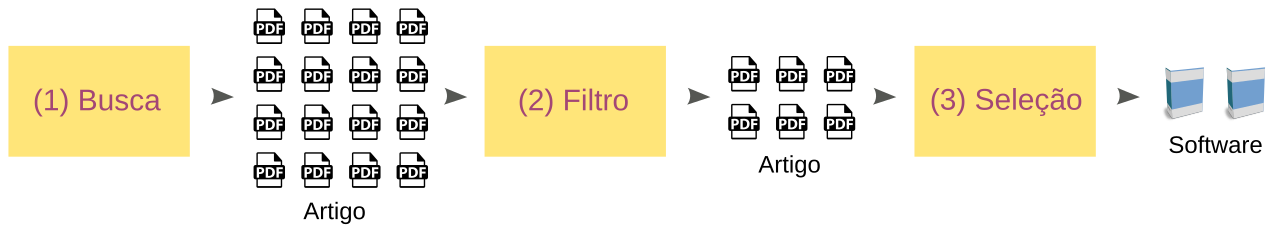
\includegraphics[scale=0.21]{imagens/etapas-selecao-software.png}
  \caption{Etapas da seleção de projetos de software acadêmico}
  \label{etapas-selecao-software}
\end{figure}

\subsubsection{Busca}

Nesta etapa definimos quais conferências serão utilizadas como fonte de busca
de software acadêmico de análise estática publicados pelos seus autores como
uma das contribuições do estudo.

A escolha de quais conferências farão parte desta etapa é realizada tendo em
vista aumentar e potencializar o número total de projetos selecionados e
busca-se conferências com histórico de publicações sobre o domínio de aplicação
do estudo, neste caso, análise estática.

Deve-se definir uma data final limite como critério de inclusão e exclusão,
sendo que a data inicial é determinada pelo histórico da conferência, devendo
englobar as edições iniciais até a última definido pela data limite.

Em casos de conferências tradicionais com longa data de existência, não é raro
que a conferência mude de nome ao longo de história, neste caso adotamos como
nome da conferência o nome mais recente e consideramos todos os outros nomes
que se passou como sendo de uma única conferência, ou seja, o nome mais
recente, mesmo que isto inclua conferencias distintas que tornaram-se uma em
algum momento.

Uma vez que estas fontes de busca estejam definidas copiamos localmente todas
as suas publicações em formato pdf até a data limite determinada, os artigos
são todos organizados em pastas por nome e ano da conferência e são também
registrados os títulos de cada artigo, além do nome da conferência e ano de
edição da conferência.

% DUVIDA: preciso dar detalhes sobre os arquivos, formato pdf, como organizei
%    em pastas, por ano, conferencia, etc?

% PDF 

% detalhar tudo, arquivos, planilhas, formato, 
% para coletar após alguns meses defini planilha, com os campos X Y e Z,
% é interessante para quem lê para saber, ...

% DUVIDA: usei libreoffice, preciso dar detalhes? fazer referencia ao nome do
%    arquivo, colunas, estrutura interna da planilha?

% o empacotamento do estudo vai pro apendice como eu já apontei sobre o sloccount por exemplo

\subsubsection{Filtro}

A segunda etapa realiza uma busca textual automática no conteúdo de cada artigo
em seu formato pdf buscando por um conjunto de palavras chave, este conjunto
total de palavras chave é composto por subconjuntos de palavras chave
representando cada subconjunto um dos critérios de inclusão e exclusão desta
fase.

\begin{itemize}
  \item Menciona software ou ferramenta
  \item Disponibiliza online
  \item Identifica endereço
  \item Domínio de análise estática
\end{itemize}

Se um artigo não satisfaz um ou mais de um destes critérios ele é excluído do
conjunto final. Cada critério é mapeado num conjunto de strings para compor a
busca final com todos os critérios.

O principal objetivo desta etapa é reduzir o conjunto de artigos inicial,
critérios são aplicados de forma automática em cada artigo do conjunto, o
filtro automático percorre os arquivos pdf de cada artigo, aplicando uma busca
textual em todo o conteúdo, incluindo título, resumo, corpo, referências,
apêndices, anexos e demais seções do arquivo.

Assim o conjunto inicial de artigos é dividido em dois outros subconjunto, um
contendo artigos sem ocorrencia dos termos relacionados aos critérios de
interesse, e outro subconjunto, passado para a etapa seguinte, com artigos
contendo os termos pesquisados.

\subsubsection{Seleção}

Nesta etapa cada artigo deste subconjunto foi lido com objetivo de identificar
através de inspeção manual se entre as contribuições do estudo há menção a
software acadêmico de análise estática, identificado minimamente com nome e URL
para obtenção online. 
Essa leitura foi guiada pelos critérios descritos na Tabela \ref{criterios-selecao}.

% DUVIDA: tenho evitado usar o termo download, isso é necessário?

\begin{table}[h]
\caption{Critério de seleção de software acadêmico}
\centering
\begin{tabular}{ l p{12cm} }
  \hline
  Critério         & Explicação \\
  \hline
  Identificável    & É possível identificar uma contribuição em software? (ex: ``um programa que nós escrevemos``, ``nossa implementação``, ``nosso protótipo'') \\
  Disponível       & Podemos encontrar a URL do software para obtenção online (download)? \\
  \hline
\end{tabular}
\label{criterios-selecao}
\end{table}

Estes critérios foram utilizados durante a inspeção de cada artigo, sendo
realizado de forma sequencial entre cada edição de cada conferência, iniciando
pelos resultados de uma certa conferência e à seguir às demais, uma por vez, de
forma crescente, ou seja, primeiro a primeira edição de uma dada conferência,
por último a última edição, em seguida, a próxima conferência, até esgotar cada
artigo de cada conferência.

%1 seleciona um artigo do conjunto e abre o arquivo pdf deste artigo
%2 busca nome do software mencionado como de autoria desta publicação
%  se encontrar toma nota do nome, artigo, conferência e passa pro próximo passo
%  se não encontrar marca artigo como não publica software e passa pro próximo artigo
%3 busca URL e identificação sobre disponibilidade do software para obtenção
%  se encontrar toma nota da URL e passa pra próxima etapa
%  se não encontrar marca artigo como não indica fonte URL para obtenção do software
%4 registra informações sobre o artigo e sobre o projeto, seleciona próximo artigo

A inspeção manual de cada artigo foi realizado através da leitura do título,
introdução, resultados e conclusão, inicialmente, caso não seja suficiente para
identificar os critérios definidos na Tabela \ref{criterios-selecao} utilizamos
as demais seções do artigo. Alguns artigos descrevem a contribuição de software
acadêmico em seções específicas, por exemplo, é comum o uso de notas de rodapé
para indicar a URL do software.

% DUVIDA: é necessário citar o nome do software que usei para ler o PDF? Evince?
%         (pode fazer diferença, mas não é necessário dar detalhes)

Os artigos inspecionados, tenha passado ou não nos critérios definidos aqui,
tiveram seus títulos, conferência, ano da conferência e uma informação
indicando se atenderam ou não os critérios, aqueles artigos que passaram nos
critérios, gera conjunto de projetos de software acadêmico com todos esses
dados e mais nome e URL do software, como mostra a Tabela \ref{esquema-selecao}.

\begin{table}[h]
\caption{Esquema para identificação do software na fase de seleção}
\centering
\begin{tabular}{ l p{11cm} }
  \hline
  Código                   & Explicação \\
  \hline
  Nome do software         & O nome do projeto de software \\
  URL                      & Endereço web do software ou projeto, site ou repositório de código fonte, com o software disponível \\
  Título do artigo         & Título do artigo onde o software é citado como contribuição, seja principal ou secundária \\
  Nome do evento           & Nome da conferência onde o software foi publicado \\
  Ano do evento            & Ano da edição da conferência onde o artigo foi publicado \\
  \hline
\end{tabular}
\label{esquema-selecao}
\end{table}

Os critérios de seleção da Tabela \ref{criterios-selecao} e o esquema para
identificação dos projetos de software apresentados na Tabela
\ref{esquema-selecao} foram adaptados do trabalho de
\citeonline{howison2016software}, que fez uma revisão de literatura da Biologia
em busca de menções a software acadêmico para evidenciar problemas de
visibilidade e de uso.

% }}}

\subsection{Caracterização dos projetos de software acadêmico de análise estática} % {{{

Os projetos de software acadêmico de análise estática selecionados foram então
caracterizados com informações adicionais coletadas por meio de inspeção manual
no website do projeto, de documentos, manuais e artigos. Quando o código fonte
estava disponível, o código fonte foi explorado em busca de informações sobre
licença, tipo de entrada e linguagens suportadas. Estas características são apresentadas
na Tabela \ref{esquema-caracteristicas}.

%foram coletadas 
%por meio de inspeção manual no website do projeto, de documentos, manuais e artigos.
%Quando o código fonte estava disponível, o código fonte foi explorado em busca de 
%informações sobre licença, tipo de entrada e linguagens suportadas.

\begin{table}[h]
\caption{Esquema para caracterização dos projetos de software selecionados}
\centering
\begin{tabular}{ l p{11cm} }
  \hline
  Característica           & Explicação \\
  \hline
  Descrição do software    & A descrição do projeto de software \\
  Acesso                   & Podemos acessar a URL do projeto agora? Pode receber os seguintes valores: Sem Acesso, Acesso Pago, Acesso Gratuito \\
  Distribuição             & Como o software é distribuído e pode ser acessado? Pode receber os seguintes valores: gratis, livre, proprietário \\
  Código fonte disponível  & É possível acessar o código fonte de alguma forma? \\
  Licença                  & O software deixa explícito qual licença é distribuído? \\
%  Permissão para modificar & Os criadores dão permissão para modificar o programa (se não menciona modificação, assume não)?; se permissão apenas por contato, também não \\
  Código fonte             & Em qual linguagem de programação o software acadêmico foi desenvolvido \\
  Entradas suportadas      & Qual o tipo de entrada suportada pelo software de análise estática \\
  Linguagens suportadas    & Quais linguagens de programação o software de análise estática suporta como entrada \\
  \hline
\end{tabular}
\label{esquema-caracteristicas}
\end{table}

Cada uma dessas características foram coletadas manualmente, primeiro
inspecionando o site do projeto, quando disponível, alguns projetos
disponibilizam manuais e documentos em seu site para download, estes documentos
foram consultados, normalmente arquivos txt, pdf ou doc. Quando disponível,
o código fonte também foi inspecionado em busca de informações, alguns projetos
distribuem junto ao código fonte documentos e manuais, outros documentam
algumas informações no próprio código fonte.

A característica sobre em qual linguagem de programação o projeto está escrito
foi coletado com o uso da ferramenta de software livre {\it
sloccount}\footnote{http://www.dwheeler.com/sloccount}, muitos projetos são
escritos em mais de uma linguagem, nestes casos consideramos a linguagem
dominante, o sloccount produz um resultado indicando todas as linguagens e
quanto do código total é escrito em cada uma delas.

% }}}

\section{Preparação} \label{estudo1:preparacao}

\subsection{Seleção dos projetos de software acadêmico de análise estática} % {{{

\subsubsection{Busca}

%pesquisa foram utilizadas como ponto de partida para
%selecionar o conjunto inicial de artigos: 
%O critério utilizado na definição destas fontes é bastante subjetivo 
%e depende de conhecimento prévio do pesquisador, seus pares, e colaboradores.

Seguindo o planejamento descrito em \ref{estudo1:planejamento}, definimos como
fonte de busca as conferências SCAM\footnote{\url{http://www.ieee-scam.org}}
({\it Source Code Analysis and Manipulation Working Conference}) e
ASE\footnote{\url{http://ase-conferences.org}} ({\it Automated Software
Engineering}), ambas conferências com um grande histórico de edições, ASE teve
sua primeira edição no ano de 1991 e o SCAM no ano de 2001, definimos como data
limite o ano de 2015, ou seja, incluimos os artigos publicados neste ano.

Ainda neste momento de preparação, buscamos descobrir onde estão disponíveis os
artigos de cada conferência e edição, as publicações da conferência SCAM, por
exemplo, estão todos disponibilizados no IEEE, ao menos até a data limite
investigada, já a conferência ASE, algumas edições está no IEEE outras só foram
encontradas na biblioteca digital da ACM, até o ano de 1996 a conferencia ASE
se chamava KBSE - Knowledge-Based Software Engineering Conference e a partir de
1997 passou a se chamar ASE - Automated Software Conference.

\subsubsection{Filtro}

1 ler sobre GQM > fechar questões de pesquisa
2 ler sobre mapeamento e revisao sistematica > revisar termos e estrutura da revisão estruturada

%Dos 346 artigos do SCAM e 1533 artigos do ASE analisados na revisão estruturada
%apenas 44\% (155 artigos) e 18\% (281 artigos) continham os termos pesquisados
%no filtro automático da segunda atividade da revisão, respectivamente.

% chris: consultar artigo de perterson para se apoiar no processo de mapeamento ou revisao sistemativa
%        tem a fase de screeming \cite{petersen2008systematic}
%        esta fase de filtro parece com a fase de screeming, ....
%        esse filtro é o screeming
% a revisao vai em profundidade lendo os artigos o mapeamento vai em largura ou abrangencia



Dando sequência a preparação do estudo, definimos as palavras chave para cada
critério de filtro, como mostra a Tabela \ref{criterios-filtro}, para definir
estas palavras chave consultamos artigos com publicação de software de análise
estática e inspecionando o seu conteúdo percebemos como usualmente os
autores mencionam contribuição em software.

% DUVIDA: qual nível de detalhe preciso dar sobre a definição destas palavras?
%         na prática, eu usei alguns artigos já conhecidos com publicação
%         de ferramenta de análise estática.

% usar termos do mapeamento e revisao, se inspirar, nao preciso me amarrar mas vou me inspirar
% o meu método vai na diagonal algo entre o mapeamento e a revisão


\begin{table}[h]
\caption{Critérios para filtro de artigos}
\centering
\begin{tabular}{ l l }
  \hline
  Critério                        & String da busca textual               \\
  \hline
  Menciona software acadêmico     & {\tt tool} ou {\tt framework}         \\
  Disponibiliza online            & {\tt download} ou {\tt available}     \\
  Identifica endereço             & {\tt http} ou {\tt ftp}               \\
  Domínio de análise estática     & {\tt static analysis} ou {\tt parser} \\
  \hline
\end{tabular}
\label{criterios-filtro}
\end{table}

Implementamos estes critérios num script e instalamos todas as dependências
necessárias para execução, todos os detalhes de instalação e forma de uso deste
script e suas dependências de execução estão documentados no Apêndice
\ref{reproducibilidade-do-estudo}.

\subsubsection{Seleção}

Nesta fase não há preparação necessária.

% }}}

\subsection{Caracterização dos projetos de software acadêmico de análise estática} % {{{

Nesta fase de preparação para caracterização dos projetos com informações
adicionais conforme planejado, definimos o formato de armazenamendo destas
informações e quais tecnologias usar para gerenciar os dados coletados, optamos
por utilizar arquivos YAML organizados em diretórios distintos para cada
projeto de software, para coletar a informação a respeito de qual linguagem de
programação o projeto está escrito, instalamos o software livre {\it
sloccount}\footnote{http://www.dwheeler.com/sloccount}, detalhes sobre o
formato YAML, estrutura utilizada para armazenamento e instalação estão
documentados no Apêndice \ref{reproducibilidade-do-estudo}.

% }}}

\section{Coleta de Dados} \label{estudo1:coleta}

Seguindo o planejamento e preparação descritos nas seções
\ref{estudo1:planejamento} e \ref{estudo1:preparacao} iniciamos a coleta dos
dados seguindo também duas grandes etapas, uma de seleção, outra de
caracterização dos projetos de software acadêmico.

\subsection{Seleção dos projetos de software acadêmico de análise estática} % {{{

A seleção dos projetos de software acadêmico de análise estática seguiu
as etapas, conforme apresentadas na Figura \ref{etapas-selecao-software}, tomando
como primeiro passo a etapa de busca.

\subsubsection{Busca}

A busca realizada nas conferências ASE e SCAM considerando todas as edições até
o ano de 2015 resultou num conjunto total de 1873 artigos, representados na
Figura \ref{artigos-por-ano} distribuídos ao longo dos anos em cada conferência.
346 artigos do SCAM e 1527 artigos do ASE,
com uma média geral de 75 artigos publicados por ano. 

\begin{figure}[h]
  \center
  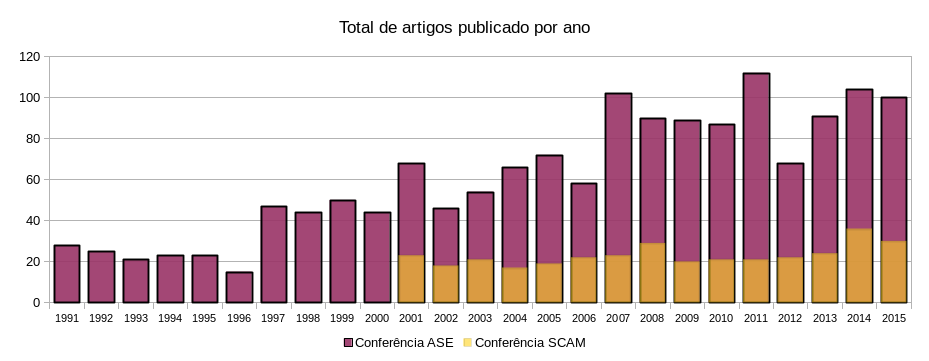
\includegraphics[scale=0.65]{imagens/artigos-por-ano.png}
  \caption{Gráfico em barras com o total de artigos publicado por ano}
  \label{artigos-por-ano}
\end{figure}

Coletamos o título de cada artigo e armazenamos juntamente com o nome da
conferência e edição onde o artigo foi publicado num arquivo do tipo ODS,
formato padrão da suíte de escritórios livre e multiplataforma
LibreOffice\footnote{\url{https://www.libreoffice.org}}, detalhes sobre este
arquivo pode ser encontrado no Apêndice \ref{reproducibilidade-do-estudo}.

\subsubsection{Filtro}

%no filtro automático da segunda atividade da revisão, respectivamente.

O filtro executado automaticamente usando os critérios definidos na fase de
preparação (seção \ref{estudo1:preparacao}) reduziu o conjunto de artigos para
441, que serão inspecionados manualmente na sequência,
155 artigos do SCAM e 286 artigos do ASE.

\subsubsection{Seleção}

Na etapa de seleção, os 441 artigos foram inspecionados, guiada pelos critérios
descritos na Tabela \ref{criterios-selecao} na fase de planejamento,
selecionados 61 artigos com publicação de software acadêmico de análise estática
segundo estes critérios, conforme Figura \ref{artigos-e-software-por-ano}
resultados distribuídos por ano.

\begin{figure}[h]
  \center
  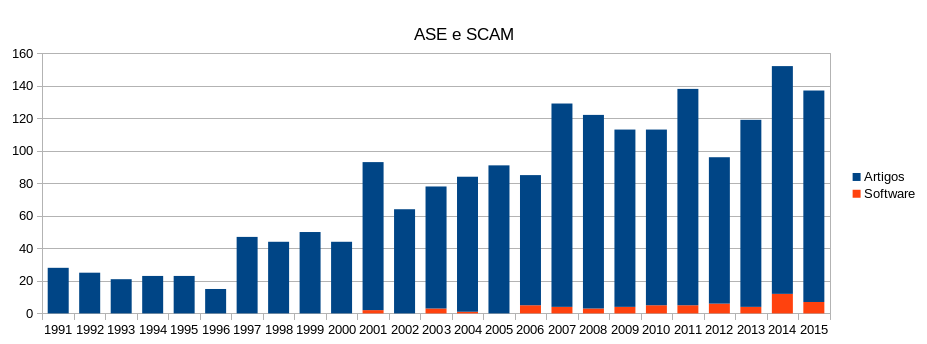
\includegraphics[scale=0.65]{imagens/artigos-e-software-por-ano.png}
  \caption{Número de projetos de software selecionados em relação ao total de publicações}
  \label{artigos-e-software-por-ano}
\end{figure}

Dois artigos, entre os 61, fazem referência a um mesmo software, assim temos no
total 60 projetos de software selecionados, para cada projeto foi criado um
diretório contendo o nome do software e um arquivo chamado
\texttt{software.yml} com os dados descritos na Tabela \ref{esquema-selecao}.

% DUVIDA: é necessário dar detalhes sobre o arquivo software.yml? sua
%         estrutura interna, quais campos, nomes dos campos.


%contribuindo com 60 projetos de software acadêmico de
%análise estática. O número de projetos de software é menor do que o número
%de artigos porque alguns foram mencionados em mais de um artigo. 

% }}}

\subsection{Caracterização dos projetos de software acadêmico de análise estática} % {{{

Conforme planejado coletamos informações adicionais para cada projeto de
software selecionado, as informações descritas na Tabela
\ref{esquema-caracteristicas} foram coletadas,

%por meio de inspeção manual no website do projeto, de documentos, manuais e artigos.
%Quando o código fonte estava disponível, o código fonte foi explorado em busca de 
%informações sobre licença, tipo de entrada e linguagens suportadas.

%Para identificar a linguagem de programação em que o software foi escrito, utilizamos a
%ferramenta livre {\it sloccount}\footnote{http://www.dwheeler.com/sloccount}.

% }}}

% \section{Operação} %%%%%%%%

% Raw results from the analysis
\section{Análise dos Dados} \label{estudo1:analise}

Dados de 60 projetos de software acadêmico de análise estática desenvolvidos e
publicados na literatura acadêmica de engenharia de software, nas conferências
ASE e SCAM, até o ano de 2015, informaçoes sobre as formas de distribuição e
licenciamento, dados de acesso ao software.

% ATENCAO: parei aqui, proximo passo:

% * criar template para gerar uma tabela e substituir a tabela (temporaria)
%   incluida abaixo
% * exibir nesta tabela as seguintes colunas para cada software:
%   - nome do software
%   - distribuição
%   - disponível para download?
%   - código fonte disponível?
%   - licença
%   - código fonte
\begin{longtable}{| l | c | c | c | c | c | c |}
\caption{Software acadêmico para análise estática.}
\label{tab:software} \\ 
  \hhline{| l | c | c | c | c | c | c |} \hline \endfirsthead
  %\hhline{|-------|} \multicolumn{7}{|c|}{continuação da página anterior} \\ \hline
  \hhline{| l | c | c | c | c | c | c |} \hline \textbf{Software} & \textbf{Versões} & \textbf{Citações} & \textbf{[cita]} & \textbf{[usa]} & \textbf{[contribui]} & \textbf{[cria]} \\ \hline
  \hhline{| l | c | c | c | c | c | c |}  \endhead
  \hhline{|-------|} \multicolumn{7}{|c|}{continua na próxima página} \\ \hline
  \hhline{|-------|} \endfoot
  \hhline{|-------|} \endlastfoot
\textbf{Software} & \textbf{Versões} & \textbf{Citações} & \textbf{[cita]} & \textbf{[usa]} & \textbf{[contribui]} & \textbf{[cria]} \\ \hline
  2ls
  &
  7
  &
  1
  &
  0
  &
  0
  &
  0
  &
  1
  \\
  accessanalysis
  &
  4
  &
  2
  &
  1
  &
  0
  &
  0
  &
  1
  \\
  apiexample
  &
  0
  &
  4
  &
  3
  &
  0
  &
  0
  &
  1
  \\
  beg
  &
  0
  &
  9
  &
  4
  &
  3
  &
  1
  &
  1
  \\
  ccjava
  &
  0
  &
  5
  &
  1
  &
  0
  &
  3
  &
  1
  \\
  civl
  &
  36
  &
  6
  &
  5
  &
  0
  &
  0
  &
  1
  \\
  codeboost
  &
  134
  &
  15
  &
  14
  &
  0
  &
  0
  &
  1
  \\
  composite
  &
  0
  &
  6
  &
  2
  &
  2
  &
  1
  &
  1
  \\
  cpa+
  &
  0
  &
  5
  &
  0
  &
  0
  &
  4
  &
  1
  \\
  cseq
  &
  0
  &
  5
  &
  1
  &
  2
  &
  1
  &
  1
  \\
  ddverify
  &
  0
  &
  3
  &
  2
  &
  0
  &
  0
  &
  1
  \\
  derailer
  &
  2
  &
  2
  &
  1
  &
  0
  &
  0
  &
  1
  \\
  diagnosys
  &
  0
  &
  1
  &
  0
  &
  0
  &
  0
  &
  1
  \\
  dompletion
  &
  0
  &
  2
  &
  1
  &
  0
  &
  0
  &
  1
  \\
  drc
  &
  0
  &
  5
  &
  4
  &
  0
  &
  0
  &
  1
  \\
  e-munity
  &
  0
  &
  1
  &
  0
  &
  0
  &
  0
  &
  1
  \\
  ejb
  &
  0
  &
  3
  &
  1
  &
  1
  &
  0
  &
  1
  \\
  error-prone
  &
  22
  &
  2
  &
  0
  &
  1
  &
  0
  &
  1
  \\
  esbmc
  &
  0
  &
  42
  &
  16
  &
  18
  &
  7
  &
  1
  \\
  etxl
  &
  0
  &
  1
  &
  0
  &
  0
  &
  0
  &
  1
  \\
  faultbuster
  &
  0
  &
  1
  &
  0
  &
  0
  &
  0
  &
  1
  \\
  flowgen
  &
  0
  &
  3
  &
  2
  &
  0
  &
  0
  &
  1
  \\
  grt
  &
  0
  &
  9
  &
  4
  &
  2
  &
  3
  &
  0
  \\
  guizmo
  &
  0
  &
  1
  &
  0
  &
  0
  &
  0
  &
  1
  \\
  gumtree
  &
  3
  &
  18
  &
  5
  &
  11
  &
  1
  &
  1
  \\
  husacct
  &
  22
  &
  7
  &
  3
  &
  2
  &
  0
  &
  2
  \\
  indus
  &
  36
  &
  4
  &
  0
  &
  3
  &
  0
  &
  1
  \\
  jastadd
  &
  24
  &
  43
  &
  24
  &
  15
  &
  3
  &
  1
  \\
  jflow
  &
  5
  &
  7
  &
  5
  &
  1
  &
  0
  &
  1
  \\
  jstereocode
  &
  0
  &
  8
  &
  2
  &
  5
  &
  0
  &
  1
  \\
  jtop
  &
  0
  &
  2
  &
  0
  &
  1
  &
  0
  &
  1
  \\
  kiasan
  &
  0
  &
  16
  &
  10
  &
  0
  &
  5
  &
  1
  \\
  loopfrog
  &
  0
  &
  5
  &
  2
  &
  2
  &
  0
  &
  1
  \\
  lotrack
  &
  0
  &
  2
  &
  1
  &
  0
  &
  0
  &
  1
  \\
  mpanalyzer
  &
  0
  &
  1
  &
  0
  &
  0
  &
  0
  &
  1
  \\
  msp
  &
  0
  &
  2
  &
  1
  &
  0
  &
  0
  &
  1
  \\
  mygcc
  &
  5
  &
  7
  &
  3
  &
  1
  &
  1
  &
  2
  \\
  parseweb
  &
  0
  &
  24
  &
  22
  &
  1
  &
  0
  &
  1
  \\
  pat
  &
  0
  &
  2
  &
  1
  &
  0
  &
  0
  &
  1
  \\
  php-air
  &
  4
  &
  9
  &
  1
  &
  5
  &
  2
  &
  1
  \\
  protopurity
  &
  0
  &
  1
  &
  0
  &
  0
  &
  0
  &
  1
  \\
  pseudogen
  &
  0
  &
  1
  &
  0
  &
  0
  &
  0
  &
  1
  \\
  ptyasm
  &
  0
  &
  2
  &
  0
  &
  0
  &
  2
  &
  0
  \\
  pumoc
  &
  0
  &
  2
  &
  1
  &
  0
  &
  0
  &
  1
  \\
  pythia
  &
  0
  &
  2
  &
  0
  &
  0
  &
  1
  &
  1
  \\
  reassert
  &
  5
  &
  13
  &
  9
  &
  3
  &
  0
  &
  1
  \\
  reve
  &
  0
  &
  1
  &
  0
  &
  0
  &
  0
  &
  1
  \\
  rrfinder
  &
  0
  &
  3
  &
  2
  &
  0
  &
  0
  &
  1
  \\
  sapid-xml
  &
  0
  &
  5
  &
  1
  &
  2
  &
  1
  &
  1
  \\
  sonarqube-plugin
  &
  4
  &
  1
  &
  0
  &
  0
  &
  0
  &
  1
  \\
  sparta
  &
  14
  &
  4
  &
  1
  &
  2
  &
  0
  &
  1
  \\
  srcml
  &
  14
  &
  40
  &
  14
  &
  23
  &
  2
  &
  1
  \\
  swat
  &
  0
  &
  4
  &
  1
  &
  2
  &
  0
  &
  1
  \\
  tacle
  &
  0
  &
  3
  &
  1
  &
  1
  &
  0
  &
  1
  \\
  teba
  &
  21
  &
  1
  &
  0
  &
  0
  &
  0
  &
  1
  \\
  testera
  &
  0
  &
  23
  &
  17
  &
  5
  &
  0
  &
  1
  \\
  vdiff
  &
  0
  &
  5
  &
  4
  &
  0
  &
  0
  &
  1
  \\
  wala
  &
  37
  &
  11
  &
  5
  &
  5
  &
  0
  &
  1
  \\
  wrangler
  &
  34
  &
  33
  &
  16
  &
  10
  &
  6
  &
  1
  \\
  xogastan
  &
  0
  &
  5
  &
  4
  &
  0
  &
  0
  &
  1
  \\
  \hline
\end{longtable}




% Hypothesis rejection
\section{Interpretação dos Resultados} \label{estudo1:interpretacao}

\subsection{Q1 - \EstudoUmQuestaoUm} % {{{

Até o ano de 1996 a conferencia ASE chamava-se KBSE\footnote{ Knowledge-Based
Software Engineering Conference} e só a partir de 1997 mudou para ASE, a
conferência SCAM teve sua primeira edição apenas em 2001, 10 anos após a
primeira edição do ASE.

No geral, a conferência ASE publica quase 4 vezes mais do que a conferência
SCAM, a edição com o maior número de publicações foi 2011 com 112 artigos
publicados, seguido de 2014 com 104, e 2007 com 102, a edição com o menor
número foi 1996 com apenas 15 artigos publicados.

Detalhes sobre o número de artigos
em cada conferência pode ser consultados nos Apêndices
\ref{artigos-do-scam} e \ref{artigos-do-ase} 

%Situação similar ocorreu com o {\it Augmenting
%Counterexample-Guided Abstraction Refinement with Proof Templates} e o {\it
%PtYasm: Software Model Checking with Proof Templates} publicados no ASE 2008,
%fazem referência ao software PtYasm. 
%Por conta disso, entre os 107 artigos, 

%Ainda durante esta última atividade da revisão cada um dos 107 artigos foram
%analisados em busca de informações sobre onde encontrar o software indicado,

Resultou em 60 softwares com indicação de fonte para obtenção do
software, apenas os artigos que indicam endereço de página web para download do
software foram selecionados, ou seja, uma grande parte dos artigos que produzem
softwares acadêmicos nem ao menos citam o software no paper, ou quando citam,
não informam site ou endereço do projeto para download
\cite{allen2017engineering}, seja código fonte ou apenas binários.


É possível perceber um crescimento no número de software publicados com o
passar dos anos, de forma que podemos confirmar que considerando as
conferências ASE e SCAM, há um crescimento na publicação de softwares
acadêmicos ao longo do tempo.

Apesar da busca na atividade -- (2) Filtro -- utilizar termos com o objetivo de
encontrar apenas softwares disponíveis com informação de onde encontrar o
software, ainda assim, encontramos 45 artigos com publicação de software sem
indicação de fonte para obtenção.

Entre os 1873 artigos, encontramos 107 artigos referenciando 105 softwares de
análise estática, apenas 60 destes indicam a fonte onde o software pode ser
encontrado.

% }}} Q1

\subsection{Q2 - \EstudoUmQuestaoDois} % {{{

%\citeonline{robles2010replicating} afirma que existe uma tendência das páginas
%web onde os softwares estão disponíveis tem uma grande chance de se tornarem
%indisponíveis ao passar do tempo, investigamos esta tendência 
%cruzando a informação de acesso ao software com a data de publicação do paper
%onde o software foi selecionado.
%a Figura \ref{softwares-disponivel-por-ano} apresenta em cada ano quantos
%porcentos do total de softwares publicados ainda continuam
%disponíveis hoje.

Apenas 37 estão disponíveis, os 23 restantes indicam fonte não mais
acessíveis, endereço não encontrado, indisponível, ou com informações não
relacionadas ao software. 
O Apêndice \ref{resumo-softwares-disponiveis} traz
uma tabela com os nomes e endereços web onde os softwares estão disponíveis.

%Levando em conta a sustentabilidade técnica podemos responder que 
Observamos que 61\% do software acadêmico produzido no domínio de aplicação de análise estática 
são sustentáveis, ou seja, continuam disponíveis ao longo do tempo. 
É importante destacar que não foram considerados aqui artigos que publicaram software 
sem menção à fonte onde o mesmo poderia ser encontrado.
% a revisão estruturada teve como foco encontrar artigos com publicação softwares com indicação de fonte,
% ou seja, aqueles artigos que publicam software mas que não indicam fonte não está sendo
% considerado aqui, vimos que na revisão estruturada, mesmo não sendo o objetivo
Se os artigos que não indicaram a fonte onde o software acadêmico poderia ser encontrado
fossem incluídos -- 45 artigos sem informação de fonte --, 
a taxa de sustentabilidade cairia para apenas 35\%.
Uma revisão estruturada mais abrangente, que desconsiderasse o critério de exclusão
(indicar fonte do software acadêmico), possivelmente resultaria em taxas abaixo dos 35\%, 
sugerindo que a quantidade de software acadêmico publicado em artigos porém indisponível para acesso
pode ser maior do que a encontrada neste estudo.

%TRABALHO FUTURO
%\citeonline{robles2010replicating} afirma que as páginas
%web onde os projetos de software acadêmico foram publicados 
%se tornem indisponíveis com o passar do tempo.
%Podemos investigar esta tendência avaliando os 60 softwares com fonte indicada no artigo,
%identificar se confirmamos neste contexto se com a idade do paper
%as páginas web onde os softwares são publicados tem uma grande chance de se
%tornarem indisponíveis ao passar do tempo.

\begin{figure}[h]
  \center
  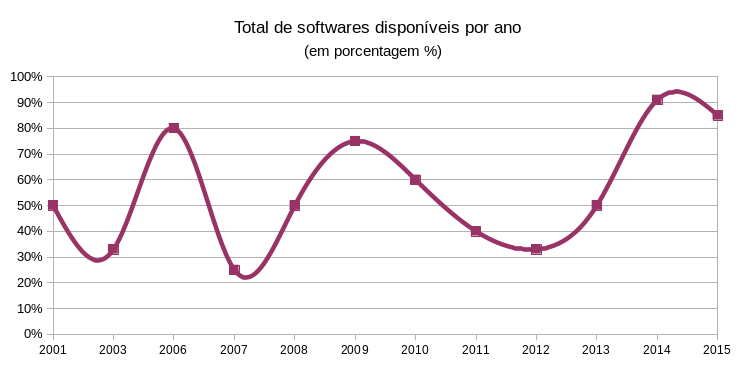
\includegraphics[scale=0.65]{imagens/softwares-disponivel-por-ano.png}
  \caption{Gráfico em linha com o total de projetos de software acadêmico disponíveis por ano}
  \label{softwares-disponivel-por-ano}
\end{figure}

A Figura \ref{softwares-disponivel-por-ano} apresenta 
um gráfico em linha com o total de projetos de software acadêmico disponíveis por ano.
Também apresenta a porcentagem de software acadêmico publicado com indicação de fonte que ainda estão
disponíveis, ou seja, a taxa de projetos de software que continuam
disponíveis hoje, considerando o conjunto de projetos de software publicado em cada ano 
com informação sobre fonte para download. 
Os anos de 2002, 2004, 2005, e anteriores a 2001 não possuem software publicado
com fonte indicada no artigo ainda disponível e, portanto,
suas informações não aparecem no gráfico.

Ao analisar a Figura \ref{softwares-disponivel-por-ano},
percebemos que há um leve crescimento na disponibilidade
dos projetos de software acadêmico  nos anos mais recentes.
%
Existe uma leve tendência, ao longo dos anos,  
para a indisponibilidade das fontes informadas e páginas web.
É possível notar que, em 2006, 80\% de todos os
softwares de análise estática publicados nas conferências ASE e SCAM ainda estão disponíveis.
Este número cresce em 2014, chegando a 90\%, e cai no ano seguinte para 85\%.
Apesar de não estar sempre crescente, e da  amostra pequena usada neste estudo 
-- apenas 60 projetos de software acadêmico,
este leve indício confirma a afirmação de \citeonline{robles2010replicating}.

Os 37 softwares com fonte disponível foram avaliados em relação ao segundo
aspecto, isto é, com respeito à forma em que estão disponíveis:
se os artigos informam onde obter tais softwares, se os softwares estão realmente disponíveis, e 
se, ao acessar as fontes indicadas na presente data deste estudo, os softwares estão funcionando e
acessíveis.

Do conjunto de 37 projetos de software estudados, %% Joenio, coloquei aqui o tempo no PRETERITO -- revisar outras partes.
3 não disponibilizaram seu código fonte e  %% Joenio, mudei as frases para VOZ ativa, sujeito: projeto de software.
34 disponibilizaram o código fonte publicamente.
Dentre os que disponibilizaram o código fonte, 13 não informaram licença alguma
%apesar de ter o código fonte disponível, 
e 21 informaram licenças de FOSS ({\it free and open source software}):

\begin{itemize}
  \item 8 usam GNU General Public License;
  \item 2 usam Apache License;
  \item 4 usam BSD License;
  \item 3 usam Eclipse Public License;
  \item 2 usam University of Illinois/NCSA Open Source License;
  \item 1 usa licença {\it FrontEndART Software Ltd}; e
  \item 1 usa licença {\it SAnToS Laboratory Open Academic License}.
\end{itemize}

Entre os 37 softwares disponíveis, 21 podem ser modificados para se adaptar às
necessidades emergentes sem necessidades de solicitação prévia de autorização
aos autores originais devido ao uso de licenças livres. 
Os 13 softwares restantes com código fonte disponível mas sem licença expressa podem
ser modificados, mas a falta de uma licença impõe a necessidade
de solicitar permissão aos autores originais.

35\% dos softwares disponíveis podem ser adaptados de forma incremental para
aproveitar oportunidades emergentes, 21\% podem mediante prévia autorização do
autor original serem modificados, e apenas 5\% não oferecem essa possibilidade
por não disponibilizarem o código fonte publicamente.

%4º Princípio, Persistencia.    % ??????

Os identificadores únicos e metadados descrevendo o software e sua disposição
devem persistir - mesmo além do tempo do software que descrevem.

%Deste total apenas 11\% (41 artigos) e 4\% (62 artigos) foram selecionados na
%terceira e última atividade da revisão contendo publicação de ferramenta de
%análise estática.

%Resultando em 103 artigos com publicação de {\it software científico} de
%análise estática de código fonte, apenas 35 possuem fonte para obtenção do
%software, sendo 32 de código aberto, ou seja, com disponibilidade de
%código fonte, e 3 grátis, apenas binários disponível. Ou seja, apenas 31\% dos
%artigos com publicação de software disponibilizam o código fonte das mesmas.
%Isto significa que 69\% dos artigos com publicação de software de análise
%estática de código fonte são potencialmente impossíveis de serem repetidos, já
%que os artefatos originais são necessários para tal atividade e o artigo não
%disponibiliza o código fonte dos mesmos.

% }}} Q2

\subsection{Q3 - \EstudoUmQuestaoTres} % {{{

Número de menções a cada software acadêmico e qual o contexto e tipo de menção
é feita, quem e quantos são os autores de cada menção.

...

%cada citação pontua no máximo 1 ponto para o peso final do paper ao quanto
%contribui para a sustentabilidade técnica do software, esta pontuação será
%calculada com base nos pesos (em porcentagem) 'contribution\_weight' e
%'authorship\_weight', este último valor é aplicado à contribution weight,
%ou seja contribution\_weight é acrescido a partir do valor de authorship\_weight.
%o valor final se ultrapassar 1 será cortado no limite 1 (máximo), a ideia não é muito
%os números, não queremos saber se são numeros altos, queremos constancia, queremos
%medir se existe um nível de contribuição mínimo aos softwares, isto está
%sendo proposto como algo que mantém o software vivo e útil para a comunidade
%acadêmmica. (por hora o valor mínimo "ideal" por ano é "0.5", ou seja, um
%valor bem modesto, este valor indica que houve ao menos uma contribuição
%ao software, ou que teve citações suficientes equivalente a uma contribuição,
%o software ao ser muito citado ganha mais visibilidade, impacta na possibilidade
%de maior adoção e maior contribuição por terceiros.

% }}} Q3

\subsection{Ameaças à validade}

Validade de construção.
A leitura dos artigos na revisão estruturada para identificar se publicam
softwares de análise estática de código fonte, se disponibilizam fonte para
obtenção de tais softwares, e se os softwares são mesmo do domínio de aplicação
de análise estática de código fonte podem ter maior validade se feitos em
par e revisados por outros pesquisadores.
Neste estudo, estas atividades foram realizadas pelo autor desta dissertação e 
não houve revisão por pesquisadores independentes.
%% A ameaça não foi tratada.

Validade externa. Apenas duas conferências. Apenas duas bases. Apenas um domínio de software acadêmico / uma área do conhecimento em que pesquisadores também programam.
%% A ameaça não foi tratada.

etapa busca: Sabemos que no subconjunto excluído, por ser automático, poderá existir artigos
dentro dos critérios mencionados, com publicação de software, mas 

\section{Conclusões} \label{estudo1:conclusoes}

FALTA uma síntese aqui. 
Este estudo ...
Resultados mostram que ...
Algumas tendências emergiram a partir da leitura ...

Planejamos fazer outro estudo ... 

% página 47 do artigo que chris vai me passar me ajuda a definir questões
% derivando do propósito, questoes sao refinamento do goals num nivel operacional
% ao responder as questões podem definir se o goal foi alcançado, verificar se
% as questões tem capacidade de responder, a questoes sao mais operacionais que
% as propostas, na capacidade de permitir a discussão se o goal foi acalçado
% ou não, se as questoes forem abstratas a interpretacao dos dados para responder
% sera dificil de entender, se sao muito detalhadas uma interpretacao clara
% nao sera possivel, para um interpretacao otima, as questoes devem ser
% definidas em um nivel intermediario de abstracao entre as metricas e o goal
% (eh util documentar as questoes formuladas) agrupar questoes similares
% vai tormar claro se a questao esta apropriada

% o core de GQM esta na parte 2 comecando no capitulo 5 (livro novo)
% ler GQM -> uso
% gqm eh generico, apesar de ser muito batido em relacao ao experimento
% ele eh util para ... melhoria de processo
% livro sobre GQM \cite{van1999goal}

%caracteriza o objeto
%  em respeito a um aspecto de qualidade
%    para determinar sua qualidade
%      sob um determinado ponto de vista
